% Capítulo 5
\chapter{Comparação de desempenho em relação ao custo de tempo e memória}
\subsection{Gráficos}
\subsubsection{Comparação do tempo esperado dos algoritmos}
O gráfico abaixo representa o tempo esperado dos três algortimos. É possível notar que o insertion-sort apresenta um tempo esperado muito maior do que os outros dois algoritmos.
\begin{figure}[h]
    \centering
    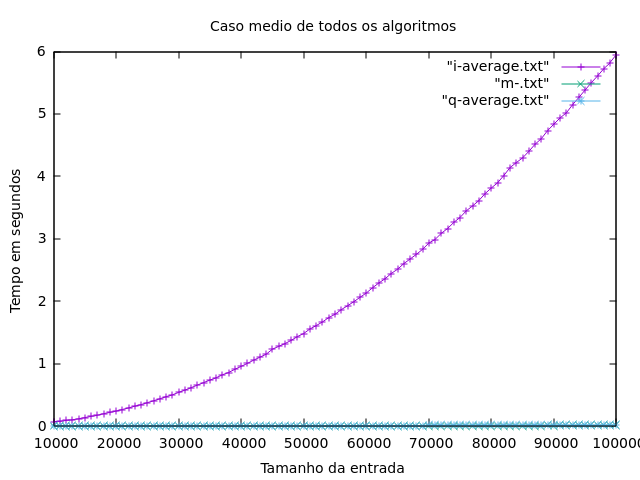
\includegraphics[width=1\linewidth]{Imagens/imq-average.png}
\end{figure}

\newpage
No gráfico abaixo excluímos o insertion-sort para podermos ver uma comparação melhor do tempo esperado do quick-sort com o tempo do merge-sort.
\begin{figure}[h]
    \centering
    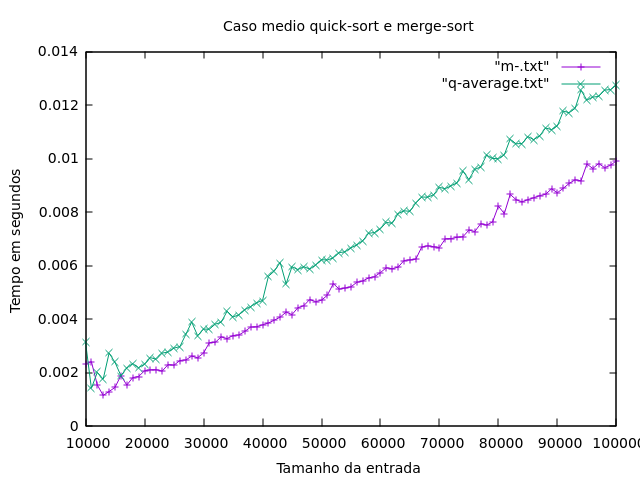
\includegraphics[width=1\linewidth]{Imagens/mq-average.png}
\end{figure}

\newpage
\subsubsection{Comparação do tempo do pior caso dos algoritmos}
Aqui abaixo temos a comparação do tempo do pior caso dos algoritmos quick-sort e insertion-sort com o o tempo do merge-sort.
\begin{figure}[h]
    \centering
    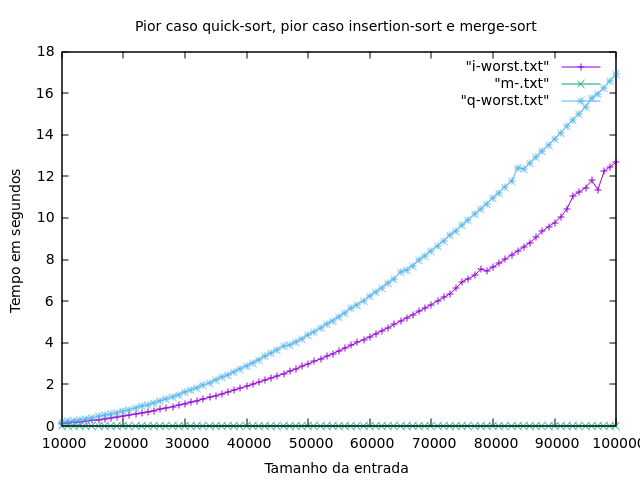
\includegraphics[width=1\linewidth]{Imagens/imq-worst.png}
\end{figure}

\newpage
\subsection{Conclusão}
Pela a análise dos gráficos de cada algoritmo levando em consideração seu melhor, pior e caso médio, foi possível observar que dentre os três, o algoritmo insertion-sort foi o que apresentou menor desempenho em relação ao tempo de execução esperado.

Porém, como não foi implementado de forma recursiva, o mesmo pode custar a menor quantidade de memória em comparação aos outros dois e seu pior caso ainda consegue ser melhor do que alguns casos específicos de pior caso do quick-sort.

Ainda analisando os algoritmos quick-sort e o merge-sort, podemos notar que, de acordo com o gráfico, o algoritmo quick-sort em seu melhor caso e seu caso médio, ainda é se apresentou rápido que o merge-sort.

Entretanto, o algoritmo merge-sort ainda se apresenta mais estável, pois, para todos os casos apresenta complexidade (n*log(n)), ao contrário do quick-sort que é volátil e mais instável, e apesar de ser mais rápido na maioria das vezes, no seu pior caso, pode chegar a complexidade de tempo O(n²), sendo bem inferior quando comparado ao tempo de execução do merge-sort.

Além disso, devemos considerar a implementação desses dois últimos de forma recursiva, que para grandes entradas podem apresentar uma sobrecarga na pilha de execução. Mas em relaçâo a memória, o quick-sort sai na frente pois o seu concorrente, o merge-sort, aloca um novo vetor a cada chamada recursiva da função merge, o que gera um gasto adicional e ainda mais notável em linguagens de mais alto nível.


\newpage
\subsubsection{Tabelas}

\centering
\caption{Melhor caso}
\begin{center}
\begin{tabular}{| l | r | r | r |}
\hline
& \multicolumn{3}{c|}{Tempo (s)}\\
\cline{2 - 4}
Tamanho da entrada & insertion-sort & merge-sort & quick-sort \\
\hline
10000 & 0.000043 & 0.002320 & 0.001124\\
20000 & 0.000057 & 0.002062 & 0.000842\\
30000 & 0.000084 & 0.002724 & 0.001341\\
40000 & 0.000126 & 0.003782 & 0.001962\\
50000 & 0.000193 & 0.004701 & 0.002213\\
\hline
\end{tabular}
\end{center}

\centering
\caption{Pior caso}
\begin{center}
\begin{tabular}{| l | r | r | r |}
\hline
& \multicolumn{3}{c|}{Tempo (s)}\\
\cline{2 - 4}
Tamanho da entrada & insertion-sort & merge-sort & quick-sort \\
\hline
10000 & 0.124559 & 0.002320 & 0.187187\\
20000 & 0.476691 & 0.002062 & 0.718812\\
30000 & 1.074601 & 0.002724 & 1.630973\\
40000 & 1.908465 & 0.003782 & 2.887971\\
50000 & 2.982496 & 0.004701 & 4.367089\\
\hline
\end{tabular}
\end{center}

\centering
\caption{Tempo esperado}
\begin{center}
\begin{tabular}{| l | r | r | r |}
\hline
& \multicolumn{3}{c|}{Tempo (s)}\\
\cline{2 - 4}
Tamanho da entrada & insertion-sort & merge-sort & quick-sort \\
\hline
10000 & 0.070669 & 0.002320 & 0.003140\\
20000 & 0.239225 & 0.002062 & 0.002307\\
30000 & 0.537542 & 0.002724 & 0.003623\\
40000 & 0.955588 & 0.003782 & 0.004691\\
50000 & 1.482152 & 0.004701 & 0.006215\\
\hline
\end{tabular}
\end{center}